\documentclass[a4paper,14pt, unknownkeysallowed]{extreport}

\usepackage{cmap} % Улучшенный поиск русских слов в полученном pdf-файле
\usepackage[T2A]{fontenc} % Поддержка русских букв
\usepackage[utf8]{inputenc} % Кодировка utf8
\usepackage[english,russian]{babel} % Языки: русский, английский
%\usepackage{pscyr} % Нормальные шрифты
\usepackage{enumitem}

\usepackage{caption}
\captionsetup{labelsep=endash}
\captionsetup[figure]{name={Рисунок}}

\usepackage{amsmath}

\usepackage{geometry}
\geometry{left=30mm}
\geometry{right=15mm}
\geometry{top=20mm}
\geometry{bottom=20mm}

\usepackage{titlesec}
\titleformat{\section}
	{\normalsize\bfseries}
	{\thesection}
	{1em}{}
\titlespacing*{\chapter}{0pt}{-30pt}{8pt}
\titlespacing*{\section}{\parindent}{*4}{*4}
\titlespacing*{\subsection}{\parindent}{*4}{*4}

\usepackage{setspace}
\onehalfspacing % Полуторный интервал

\frenchspacing
\usepackage{indentfirst} % Красная строка

\usepackage{titlesec}
\titleformat{\chapter}{\LARGE\bfseries}{\thechapter}{20pt}{\LARGE\bfseries}
\titleformat{\section}{\Large\bfseries}{\thesection}{20pt}{\Large\bfseries}

\usepackage{listings}
\usepackage{xcolor}

\lstdefinestyle{rust}{
	%language=Rust,
	backgroundcolor=\color{white},
	basicstyle=\footnotesize\ttfamily,
	keywordstyle=\color{blue},
	stringstyle=\color{red},
	commentstyle=\color{gray},
	directivestyle=\color{orange},
	numbers=left,
	numberstyle=\tiny,
	stepnumber=1,
	numbersep=5pt,
	frame=single,
	tabsize=4,
	captionpos=t,
	breaklines=true,
	breakatwhitespace=true,
	escapeinside={\#*}{*)},
	morecomment=[l][\color{magenta}]{\#},
	columns=fullflexible
}


\usepackage{pgfplots}
\usetikzlibrary{datavisualization}
\usetikzlibrary{datavisualization.formats.functions}

\usepackage{graphicx}
\newcommand{\img}[3] {
	\begin{figure}[h!]
		\center{\includegraphics[height=#1]{inc/img/#2}}
		\caption{#3}
		\label{img:#2}
	\end{figure}
}
\newcommand{\boximg}[3] {
	\begin{figure}[h]
		\center{\fbox{\includegraphics[height=#1]{inc/img/#2}}}
		\caption{#3}
		\label{img:#2}
	\end{figure}
}

\usepackage[justification=centering]{caption} % Настройка подписей float объектов

\usepackage[unicode,pdftex]{hyperref} % Ссылки в pdf
\hypersetup{hidelinks}

\usepackage{csvsimple}

\newcommand{\code}[1]{\texttt{#1}}

\begin{document}

\begin{titlepage}
	\newgeometry{pdftex, left=2cm, right=2cm, top=2.5cm, bottom=2.5cm}
	\fontsize{12pt}{12pt}\selectfont
	\noindent \begin{minipage}{0.15\textwidth}
		
\includegraphics[width=\linewidth]{images/b_logo.jpg}
	\end{minipage}
	\noindent\begin{minipage}{0.9\textwidth}\centering
		\textbf{Министерство науки и высшего образования Российской Федерации}\\
		\textbf{Федеральное государственное бюджетное образовательное учреждение высшего образования}\\
		\textbf{«Московский государственный технический университет имени Н.Э. Баумана}\\
		\textbf{(национальный исследовательский университет)»}\\
		\textbf{(МГТУ им. Н.Э.~Баумана)}
	\end{minipage}
	
	\noindent\rule{18cm}{3pt}
	\newline\newline
	\noindent ФАКУЛЬТЕТ $\underline{\text{«Информатика и системы управления»}}$ \newline\newline
	\noindent КАФЕДРА $\underline{\text{«Программное обеспечение ЭВМ и информационные технологии»}}$\newline\newline\newline\newline\newline\newline\newline
	
	
	\begin{center}
		\Large\textbf{Отчет по лабораторной работе №1 по курсу "Анализ алгоритмов"}\newline
	\end{center}
	
	\noindent\textbf{Тема} $\underline{\text{Расстояние Левенштейна и Дамерау-Левенштейна}}$\newline\newline\newline
	\noindent\textbf{Студент} $\underline{\text{Коротыч М. Д.~~~~~~~~~~~~~~~~~~~~~~~~~~~~~~~~~~~~~~~~~}}$\newline\newline
	\noindent\textbf{Группа} $\underline{\text{ИУ7-55Б~~~~~~~~~~~~~~~~~~~~~~~~~~~~~~~~~~~~~~~~~~~~~~~~~~}}$\newline\newline
	\noindent\textbf{Преподаватели} $\underline{\text{~~~~~~~~~~~~~~~~~~~~}}$\newline
	
	\begin{center}
		\vfill
		Москва~---~\the\year
		~г.
	\end{center}
 \restoregeometry
\end{titlepage}

\tableofcontents

\chapter*{Введение}
\addcontentsline{toc}{chapter}{Введение}

Расстояние Левенштейна (редакционное расстояние) — метрика, измеряющая разность между двумя последовательностями символов. Она определяется как минимальное количество односимвольных операций (вставки, удаления, замены), необходимых для превращения одной последовательности символов в другую. В общем случае, операциям, используемым в этом преобразовании, можно назначить разные цены. Широко используется в теории информации и компьютерной лингвистике.

Впервые задачу поставил в 1965 году советский математик Владимир Левенштейн при изучении последовательностей 0--1, впоследствии более общую задачу для произвольного алфавита связали с его именем.

Расстояние Левенштейна и его обобщения применяются: 
\begin{enumerate}
	\item для исправления ошибок в слове (в поисковых системах, базах данных, при вводе текста, при автоматическом распознавании отсканированного текста или речи);
	\item для сравнения текстовых файлов утилитой \code{diff} и ей подобными;
	\item в биоинформатике.
\end{enumerate}

Расстояние Дамерау — Левенштейна (названо в честь учёных Фредерика Дамерау и Владимира Левенштейна) — это мера разницы двух строк символов, определяемая как минимальное количество операций вставки, удаления, замены и транспозиции (перестановки двух соседних символов), необходимых для перевода одной строки в другую. Является модификацией расстояния Левенштейна.

Целью данной лабораторной работы является изучение, реализация и исследование алгоритмов нахождения расстояний Левенштейна и Дамерау - Левенштейна. Задачами данной лабораторной работы являются:
\begin{itemize}
    \item изучение алгоритмов нахождения расстояния Левенштейна и Дамерау - Левенштейна;
    \item сравнение и выявление достоинств и недостатков рассмотренных алгоритмов;
	\item применение методов динамического программирования для реализации алгоритмов;
	\item получение практических навыков реализации алгоритмов Левенштейна и Дамерау — Левенштейна;
	\item сравнительный анализ алгоритмов на основе экспериментальных данных;
	\item подготовка отчёта по лабораторной работе.
\end{itemize}

\chapter{Аналитическая часть}

Расстояние Левенштейна между двумя строками — это минимальное количество операций вставки, удаления и замены, необходимых для превращения одной строки в другую.

Цены операций могут зависеть от вида операции (вставка, удаление, замена) и/или от участвующих в ней символов. В общем случае имеются следующие стоимости:
\begin{itemize}
	\item $w(a, b)$ — цена замены символа $a$ на символ $b$;
	\item $w(\lambda, b)$ — цена вставки символа $b$;
	\item $w(a, \lambda)$ — цена удаления символа $a$.
\end{itemize}

Для решения задачи о редакционном расстоянии необходимо найти последовательность замен, которая минимизирует суммарную цену. Расстояние Левенштейна является частным случаем этой задачи при:
\begin{itemize}
	\item $w(a, a) = 0$;
	\item $w(a, b) = 1, \medspace a \neq b$;
	\item $w(\lambda, b) = 1$;
	\item $w(a,\lambda) = 1$.
\end{itemize}

\clearpage

\section{Рекурсивный алгоритм}

Расстояние Левенштейна между двумя строками a и b может быть вычислено по формуле \ref{eq:D}, где $|a|$ означает длину строки $a$; $a[i]$ — i-ый символ строки $a$ , функция $D(i, j)$ определена как:
\begin{equation}
	\label{eq:D}
	D(i, j) = \begin{cases}
		0 &\text{i = 0, j = 0}\\
		i &\text{j = 0, i > 0}\\
		j &\text{i = 0, j > 0}\\
		\min \lbrace \\
			\qquad D(i, j - 1) + 1\\
			\qquad D(i - 1, j) + 1 &\text{i > 0, j > 0}\\
			\qquad D(i - 1, j - 1) + m(a[i], b[j]) &\text(\ref{eq:m})\\
		\rbrace
	\end{cases},
\end{equation}

а функция \ref{eq:m} определена как:
\begin{equation}
	\label{eq:m}
	m(a, b) = \begin{cases}
		0 &\text{если a = b,}\\
		1 &\text{иначе}
	\end{cases}.
\end{equation}

Рекурсивный алгоритм реализует формулу \ref{eq:D}.
Функция $D$ составлена из следующих соображений:
\begin{enumerate}
	\item для перевода из пустой строки в пустую требуется ноль операций;
	\item для перевода из пустой строки в строку $a$ требуется $|a|$ операций;
	\item для перевода из строки $a$ в пустую требуется $|a|$ операций.
\end{enumerate}
Для перевода из строки $a$ в строку $b$ требуется выполнить некоторое количество операций (удаление, вставка, замена) в некоторой последовательности. Полагая, что $a'$, $b'$  — строки $a$ и $b$ без последнего символа соответственно, цена преобразования из строки $a$ в строку $b$ может быть выражена как:
	\begin{enumerate}
		\item сумма цены преобразования строки $a'$ в $b$ и цены проведения операции удаления, которая необходима для преобразования $a'$ в $a$;
		\item сумма цены преобразования строки $a$ в $b'$  и цены проведения операции вставки, которая необходима для преобразования $b'$ в $b$;
		\item сумма цены преобразования из $a'$ в $b'$ и операции замены, предполагая, что $a$ и $b$ оканчиваются на разные символы;
		\item цена преобразования из $a'$ в $b'$, предполагая, что $a$ и $b$ оканчиваются на один и тот же символ.
	\end{enumerate}
Минимальной ценой преобразования будет минимальное значение приведенных вариантов.

\section{Матричный алгоритм}

Прямая реализация формулы \ref{eq:D} может быть малоэффективна по времени исполнения при больших $i$, $j$, т. к. множество промежуточных значений $D(i, j)$ вычисляются заново множество раз подряд. Для оптимизации нахождения расстояния Левенштейна можно использовать матрицу для хранения соответствующих промежуточных значений. В таком случае алгоритм представляет собой построчное заполнение матрицы 
$A_{(|a| + 1)\times (|b| + 1)}$ значениями $D(i, j)$.

\section{Рекурсивный алгоритм с заполнением матрицы}
\label{sec:recmat}

Рекурсивный алгоритм заполнения можно оптимизировать по времени выполнения с использованием матричного алгоритма. Суть данного метода заключается в параллельном заполнении матрицы при выполнении рекурсии. В случае, если рекурсивный алгоритм выполняет прогон для данных, которые ещё не были обработаны, результат нахождения расстояния заносится в матрицу. В случае если обработанные ранее данные встречаются снова, для них расстояние не находится и алгоритм переходит к следующему шагу.

\section{Расстояние Дамерау — Левенштейна}

Расстояние Дамерау — Левенштейна может быть найдено по формуле \ref{eq:d}, которая задана как
\begin{equation}
	\label{eq:d}
	d_{a, b}(i, j) = \begin{cases}
		\max(i, j), &\text{если }\min(i, j) = 0,\\
		\min \lbrace \\
			\qquad d_{a, b}(i, j - 1) + 1,\\
			\qquad d_{a, b}(i - 1, j) + 1,\\
			\qquad d_{a, b}(i - 1, j - 1) + m(a[i], b[j]), &\text{иначе}\\
			\qquad \left[ \begin{array}{cc}d_{a,b}(i - 2, j - 2) + 1, &\text{если }i, j > 1;\\
			\qquad &\text{}a[i] = b[j - 1]; \\
			\qquad &\text{}b[j] = a[i - 1]\\
			\qquad \infty, & \text{иначе}\end{array}\right.\\
		\rbrace
		\end{cases},
\end{equation}

Формула выводится так же, как и формула (\ref{eq:D}).
Как и в случае с рекурсией, прямое применение этой формулы неэффективно по времени исполнения, поэтому аналогично методу из \ref{sec:recmat} добавляется матрица для хранения промежуточных значений рекурсивной формулы.

\section{Вывод}

Формулы Левенштейна и Дамерау — Левенштейна для расчёта расстояния между строками задаются рекурсивно, а следовательно, алгоритмы могут быть реализованы рекурсивно или итерационно.

% Пусть $S_{1}$ и $S_{2}$ — две строки (длиной $M$ и $N$ соответственно) над некоторым алфавитом, тогда расстояние Левенштейна $d(S_{1},S_{2})$ можно подсчитать по рекуррентной формуле $d(S_{1},S_{2}) = D(M,N)$, где\\
% \begin{equation}
% 	D(i,j) = 
% 	\left \{ \begin{aligned}
% 		& 0, & i = 0, \medspace j = 0\\
% 		& i, & i > 0, \medspace j = 0\\
% 		& j, & i = 0, \medspace j > 0\\
% 		& \min\{ &\\
% 		& \qquad D(i, j - 1) + 1, & \\
% 		& \qquad D(i - 1, j) + 1, & i > 0, \medspace j > 0\\
% 		& \qquad D(i - 1, j - 1) + m(S_{1}[i], S_{2}[j]) &\\
% 		& \} &
% 	\end{aligned} \right. 
% \end{equation}

\chapter{Конструкторская часть}

\section{Схема алгоритма нахождения расстояния Левенштейна}

На рисунке \ref{img:lev_dist_rec} приведена схема рекурсивного алгоритма нахождения расстояния Левенштейна.

\begin{figure}[hbt]
\centering
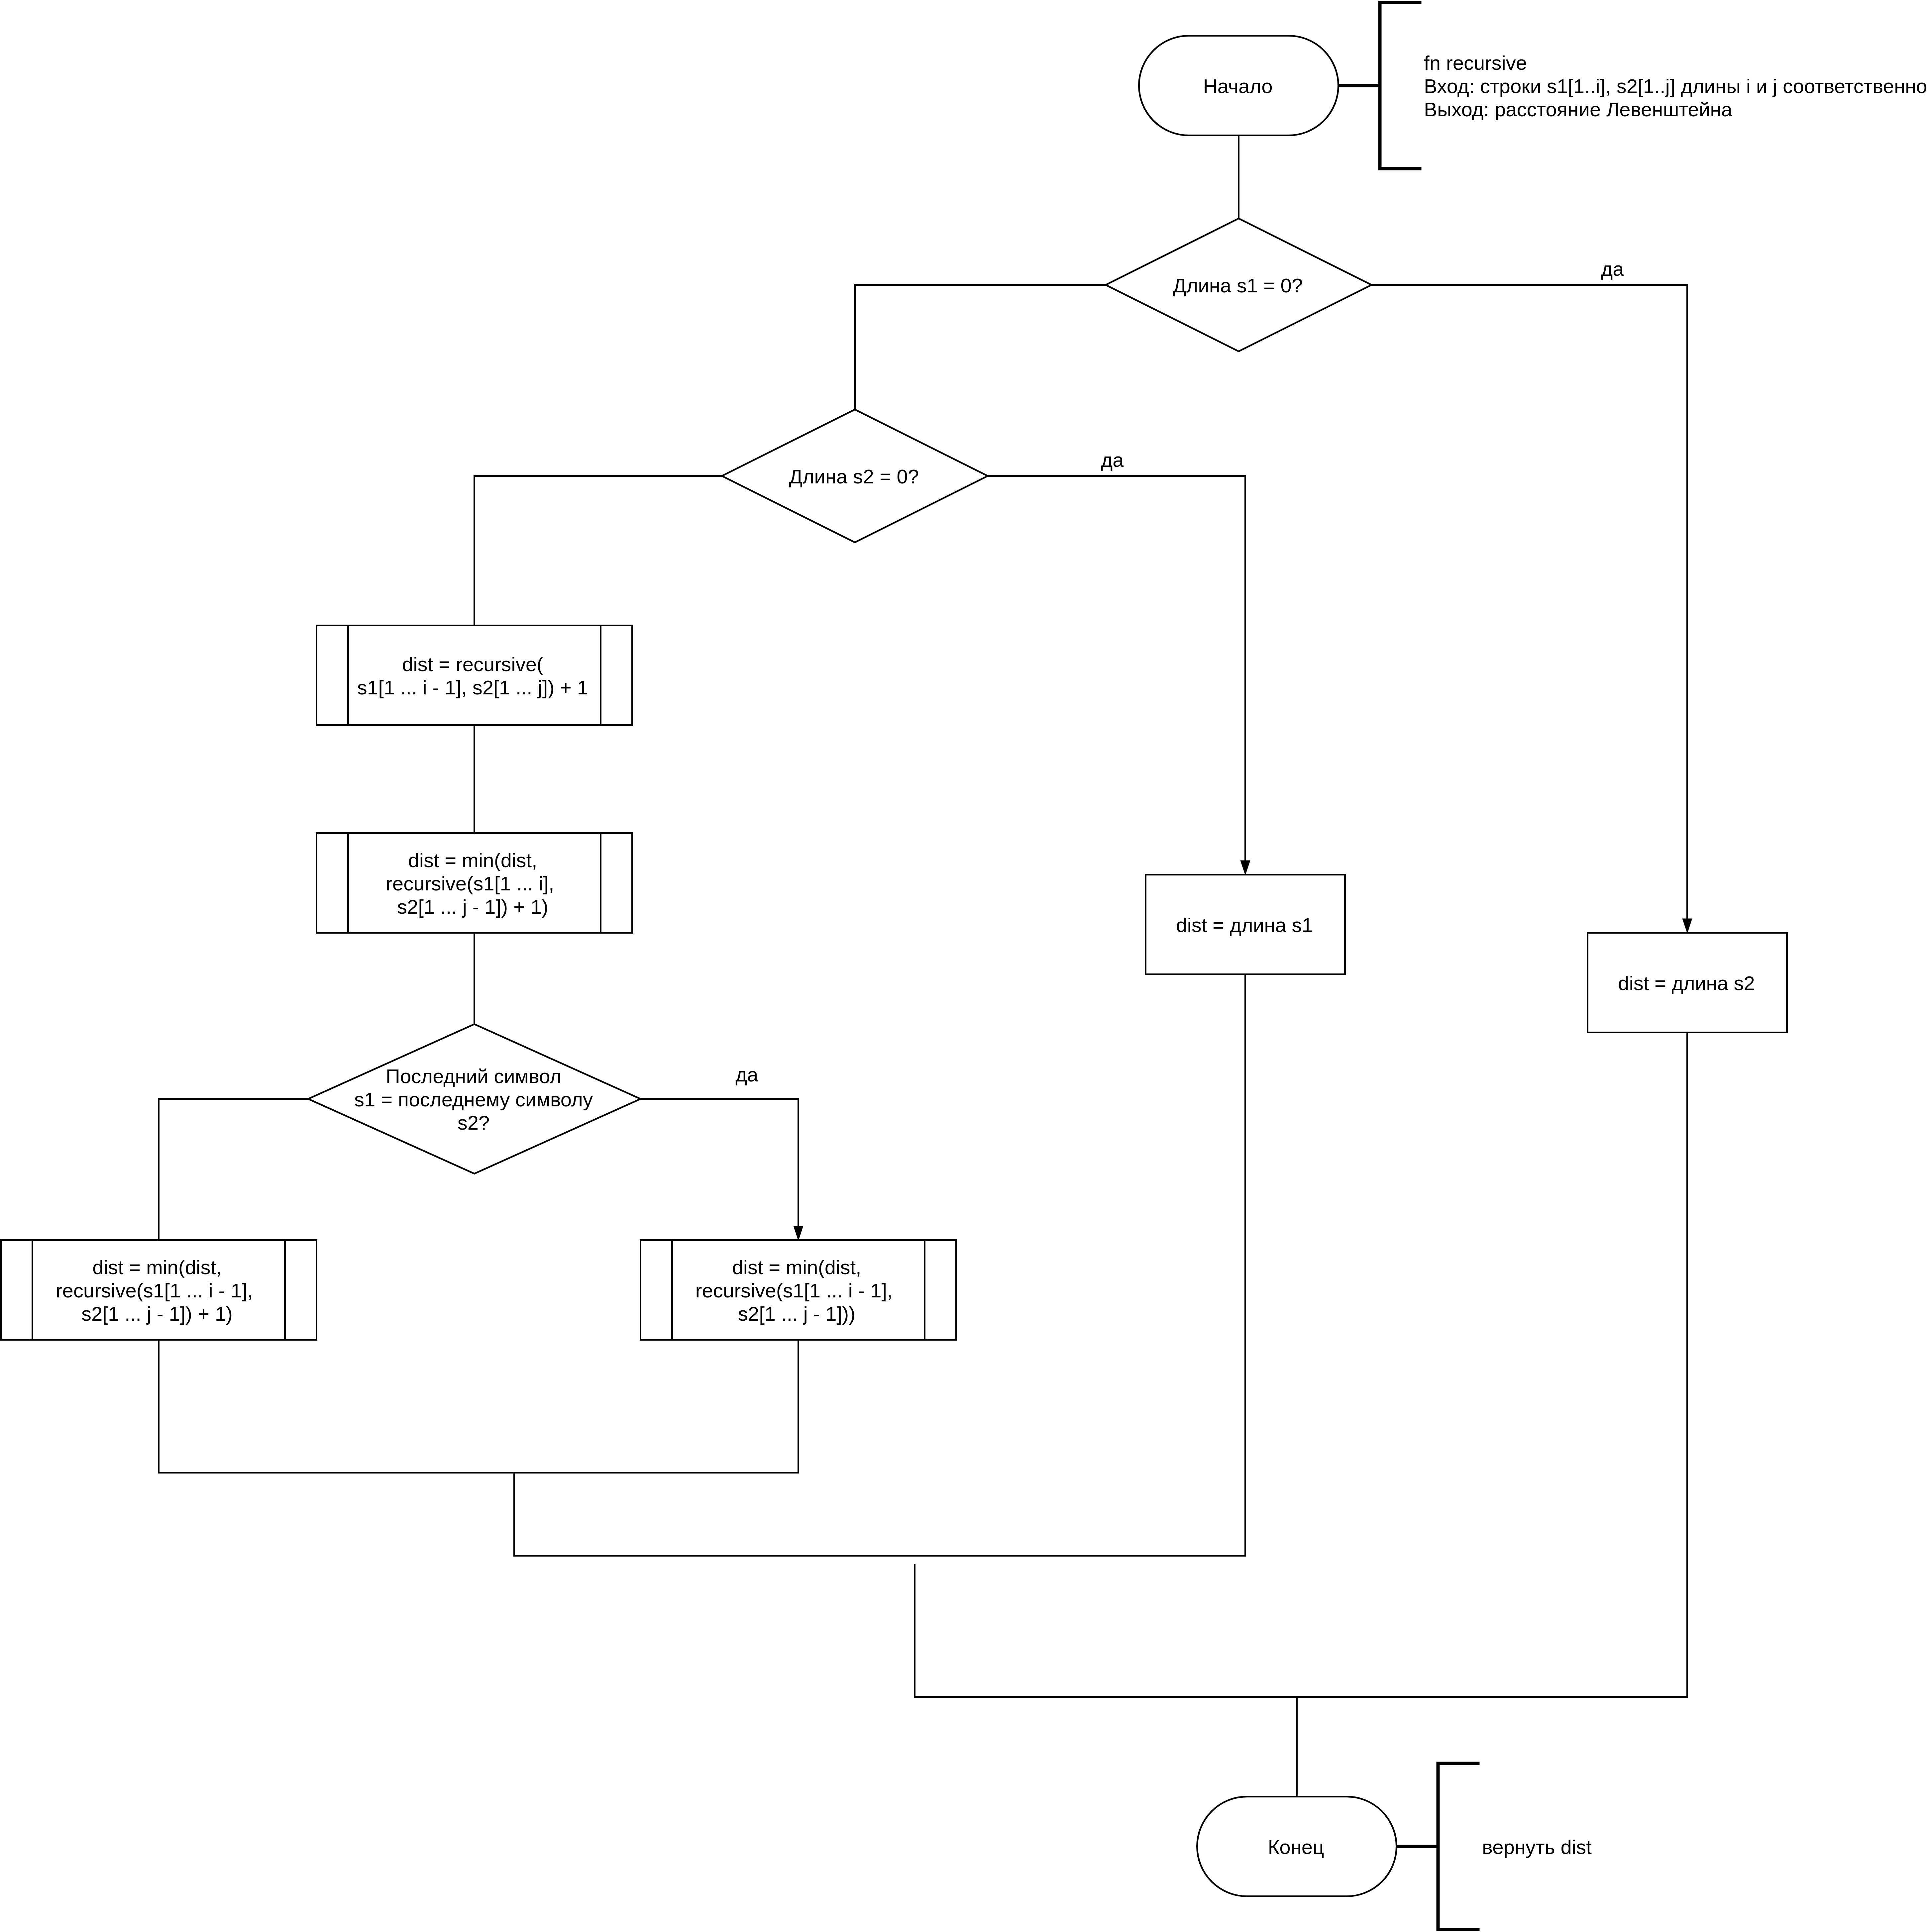
\includegraphics[width=160mm]{images/recursive.png}
\caption{Схема рекурсивного алгоритма нахождения расстояния Левенштейна}
\label{img:lev_dist_rec}
\end{figure}

На рисунке \ref{img:init_matrix} схема алгоритма инициализации матрицы.

\begin{figure}
\centering
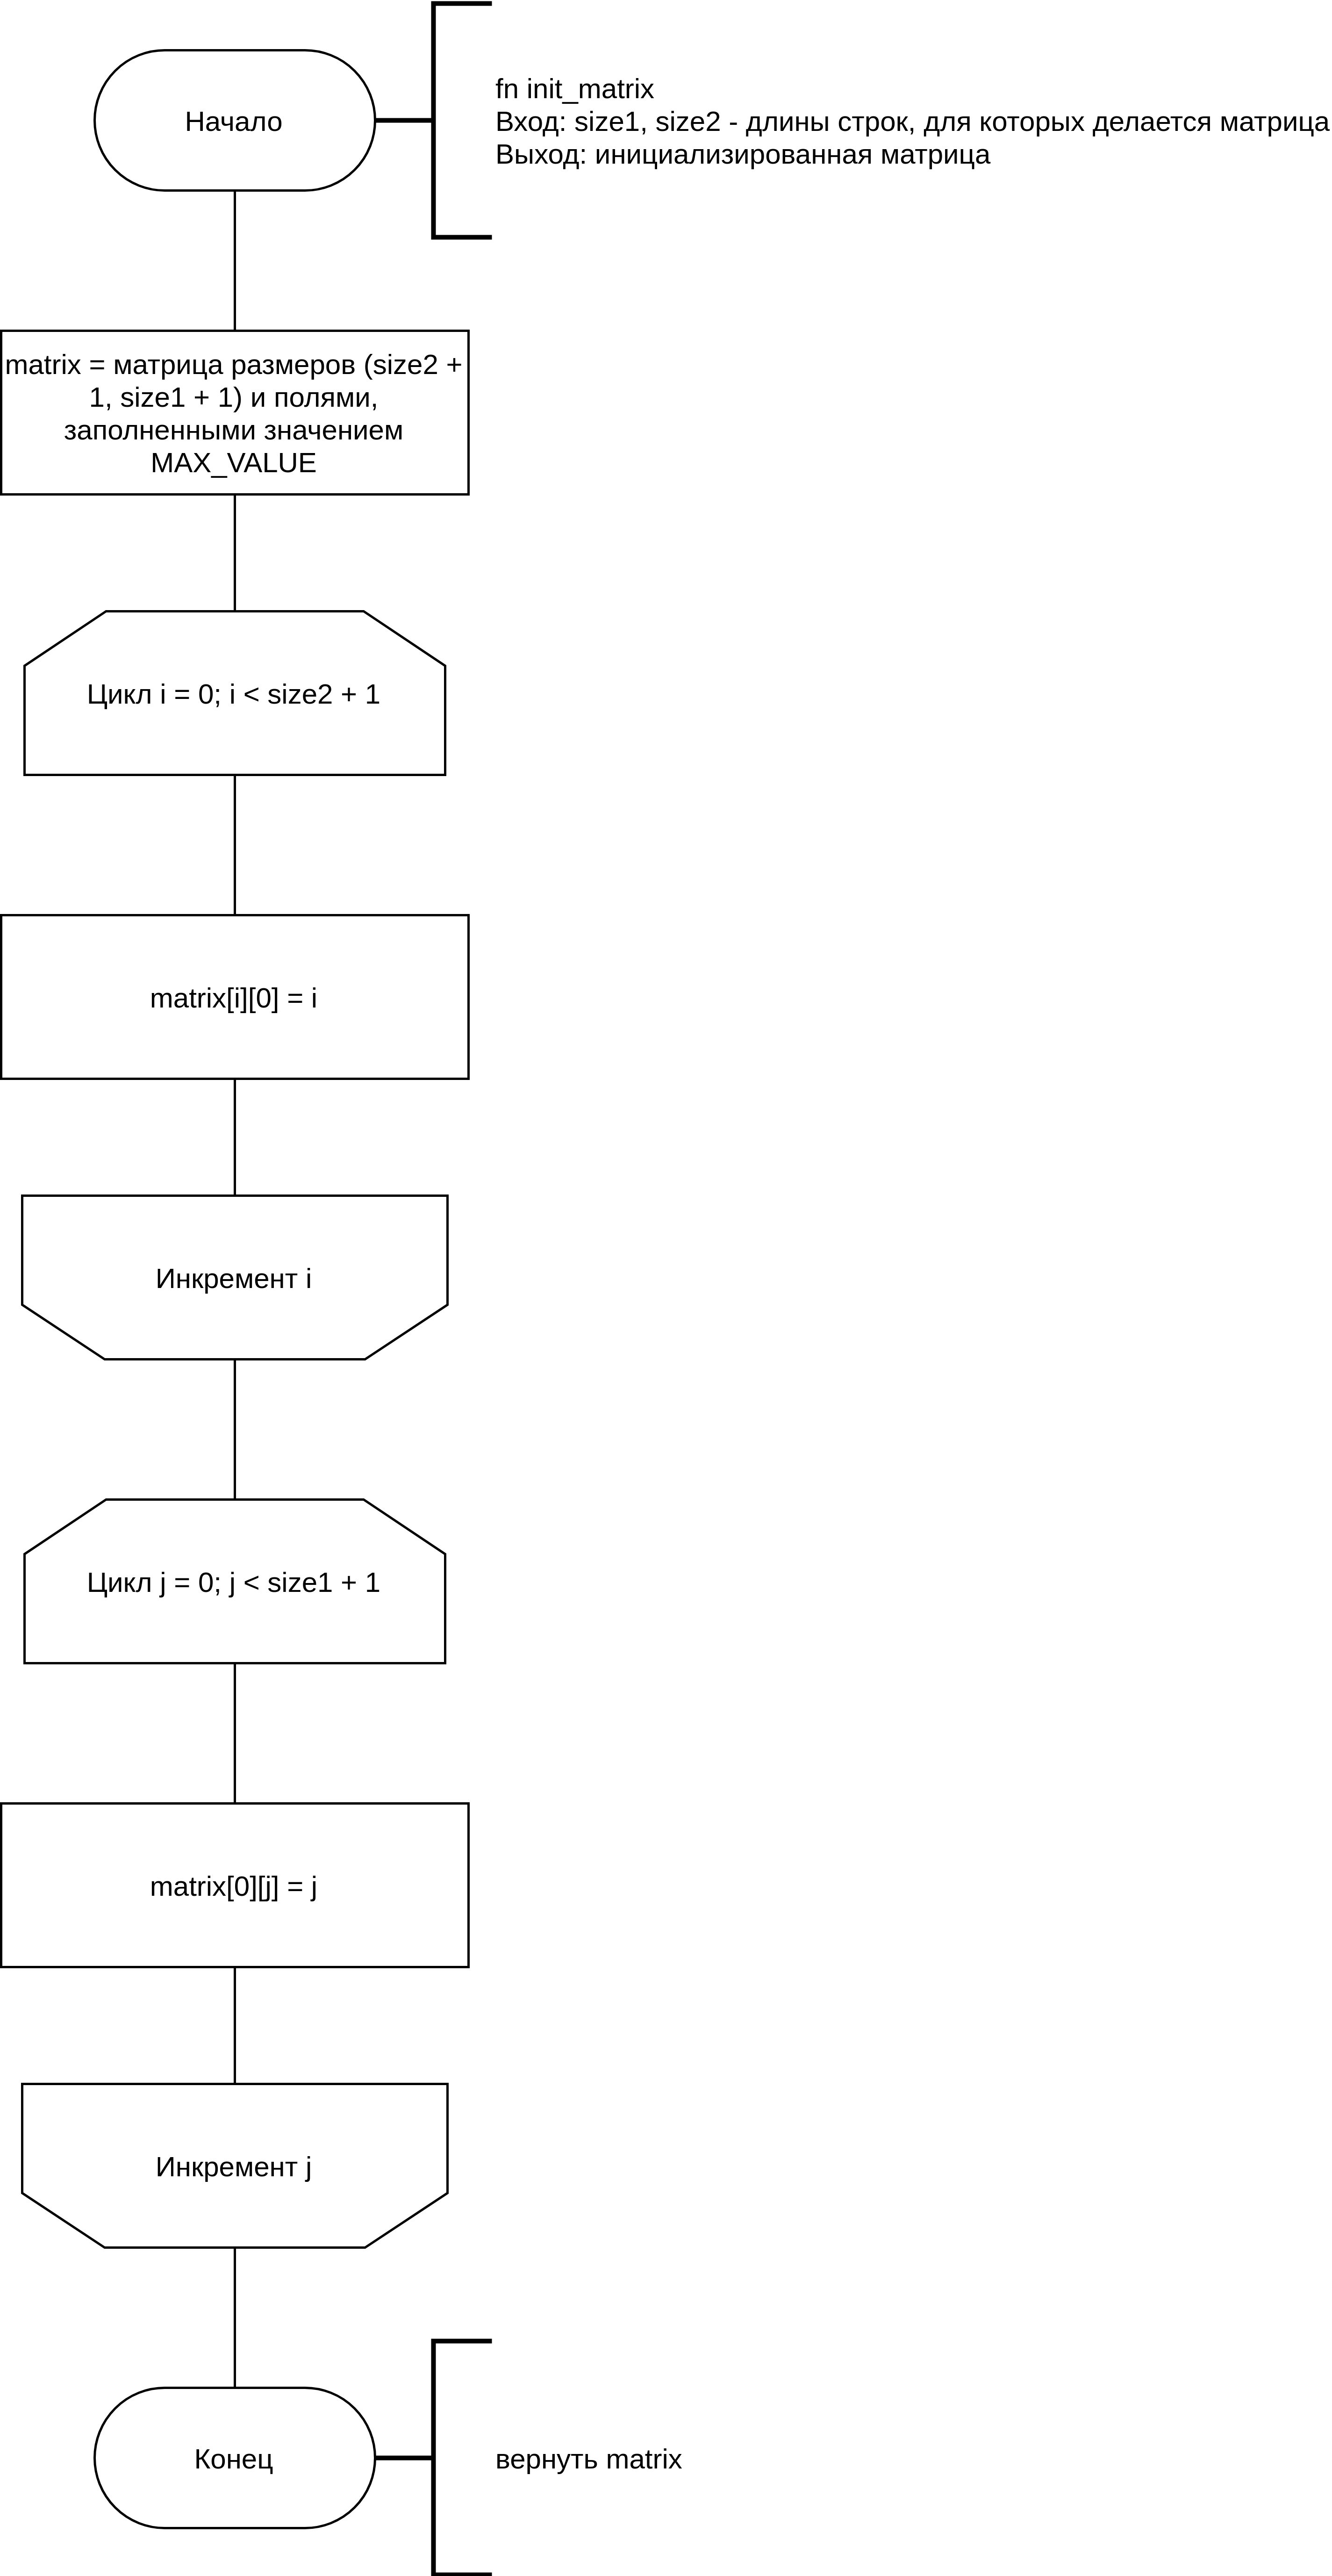
\includegraphics[width=100mm]{images/init_matrix.png}
\caption{Схема алгоритма инициализации матрицы}
\label{img:init_matrix}
\end{figure}

На рисунках \ref{img:rec_mem} и \ref{img:recursive_with_mem} приведена схема рекурсивного алгоритма нахождения расстояния Левенштейна с заполнением матрицы.

\begin{figure}[h]
\centering
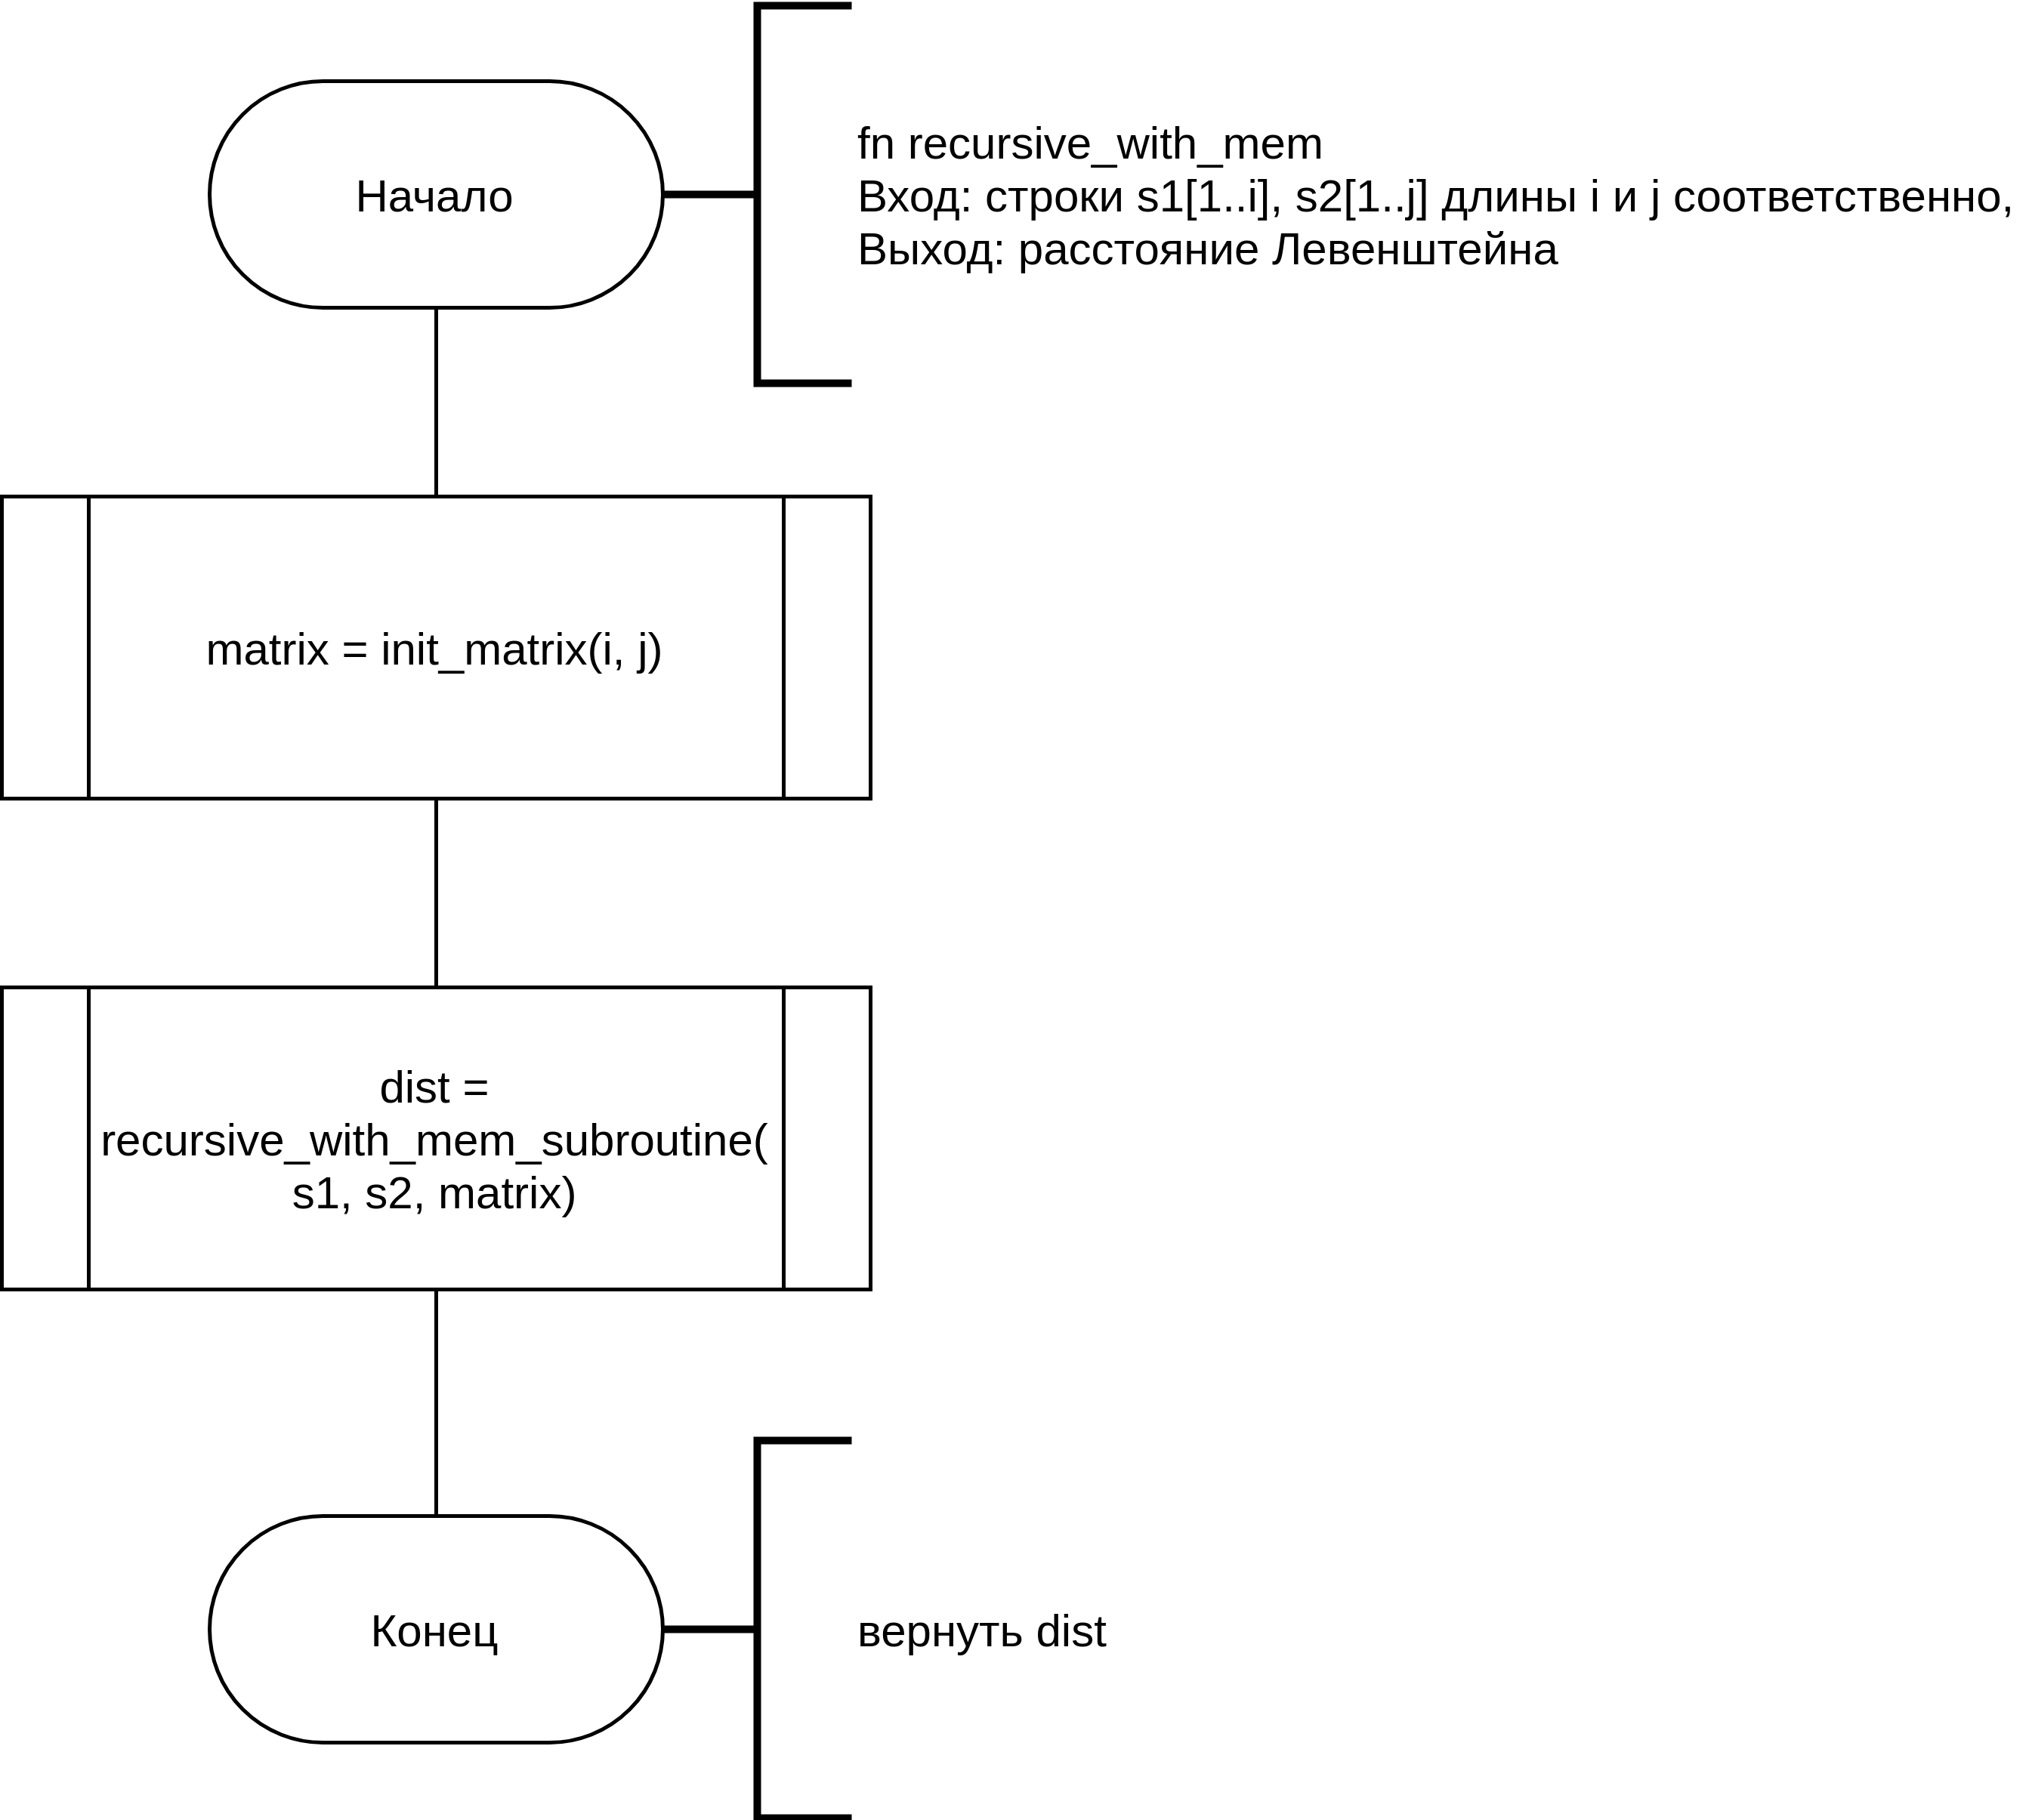
\includegraphics[width=160mm]{images/rec_mem.png}
\caption{Схема матрично-рекурсивного алгоритма нахождения расстояния Левенштейна}
\label{img:rec_mem}
\end{figure}

\clearpage

\begin{figure}
\centering
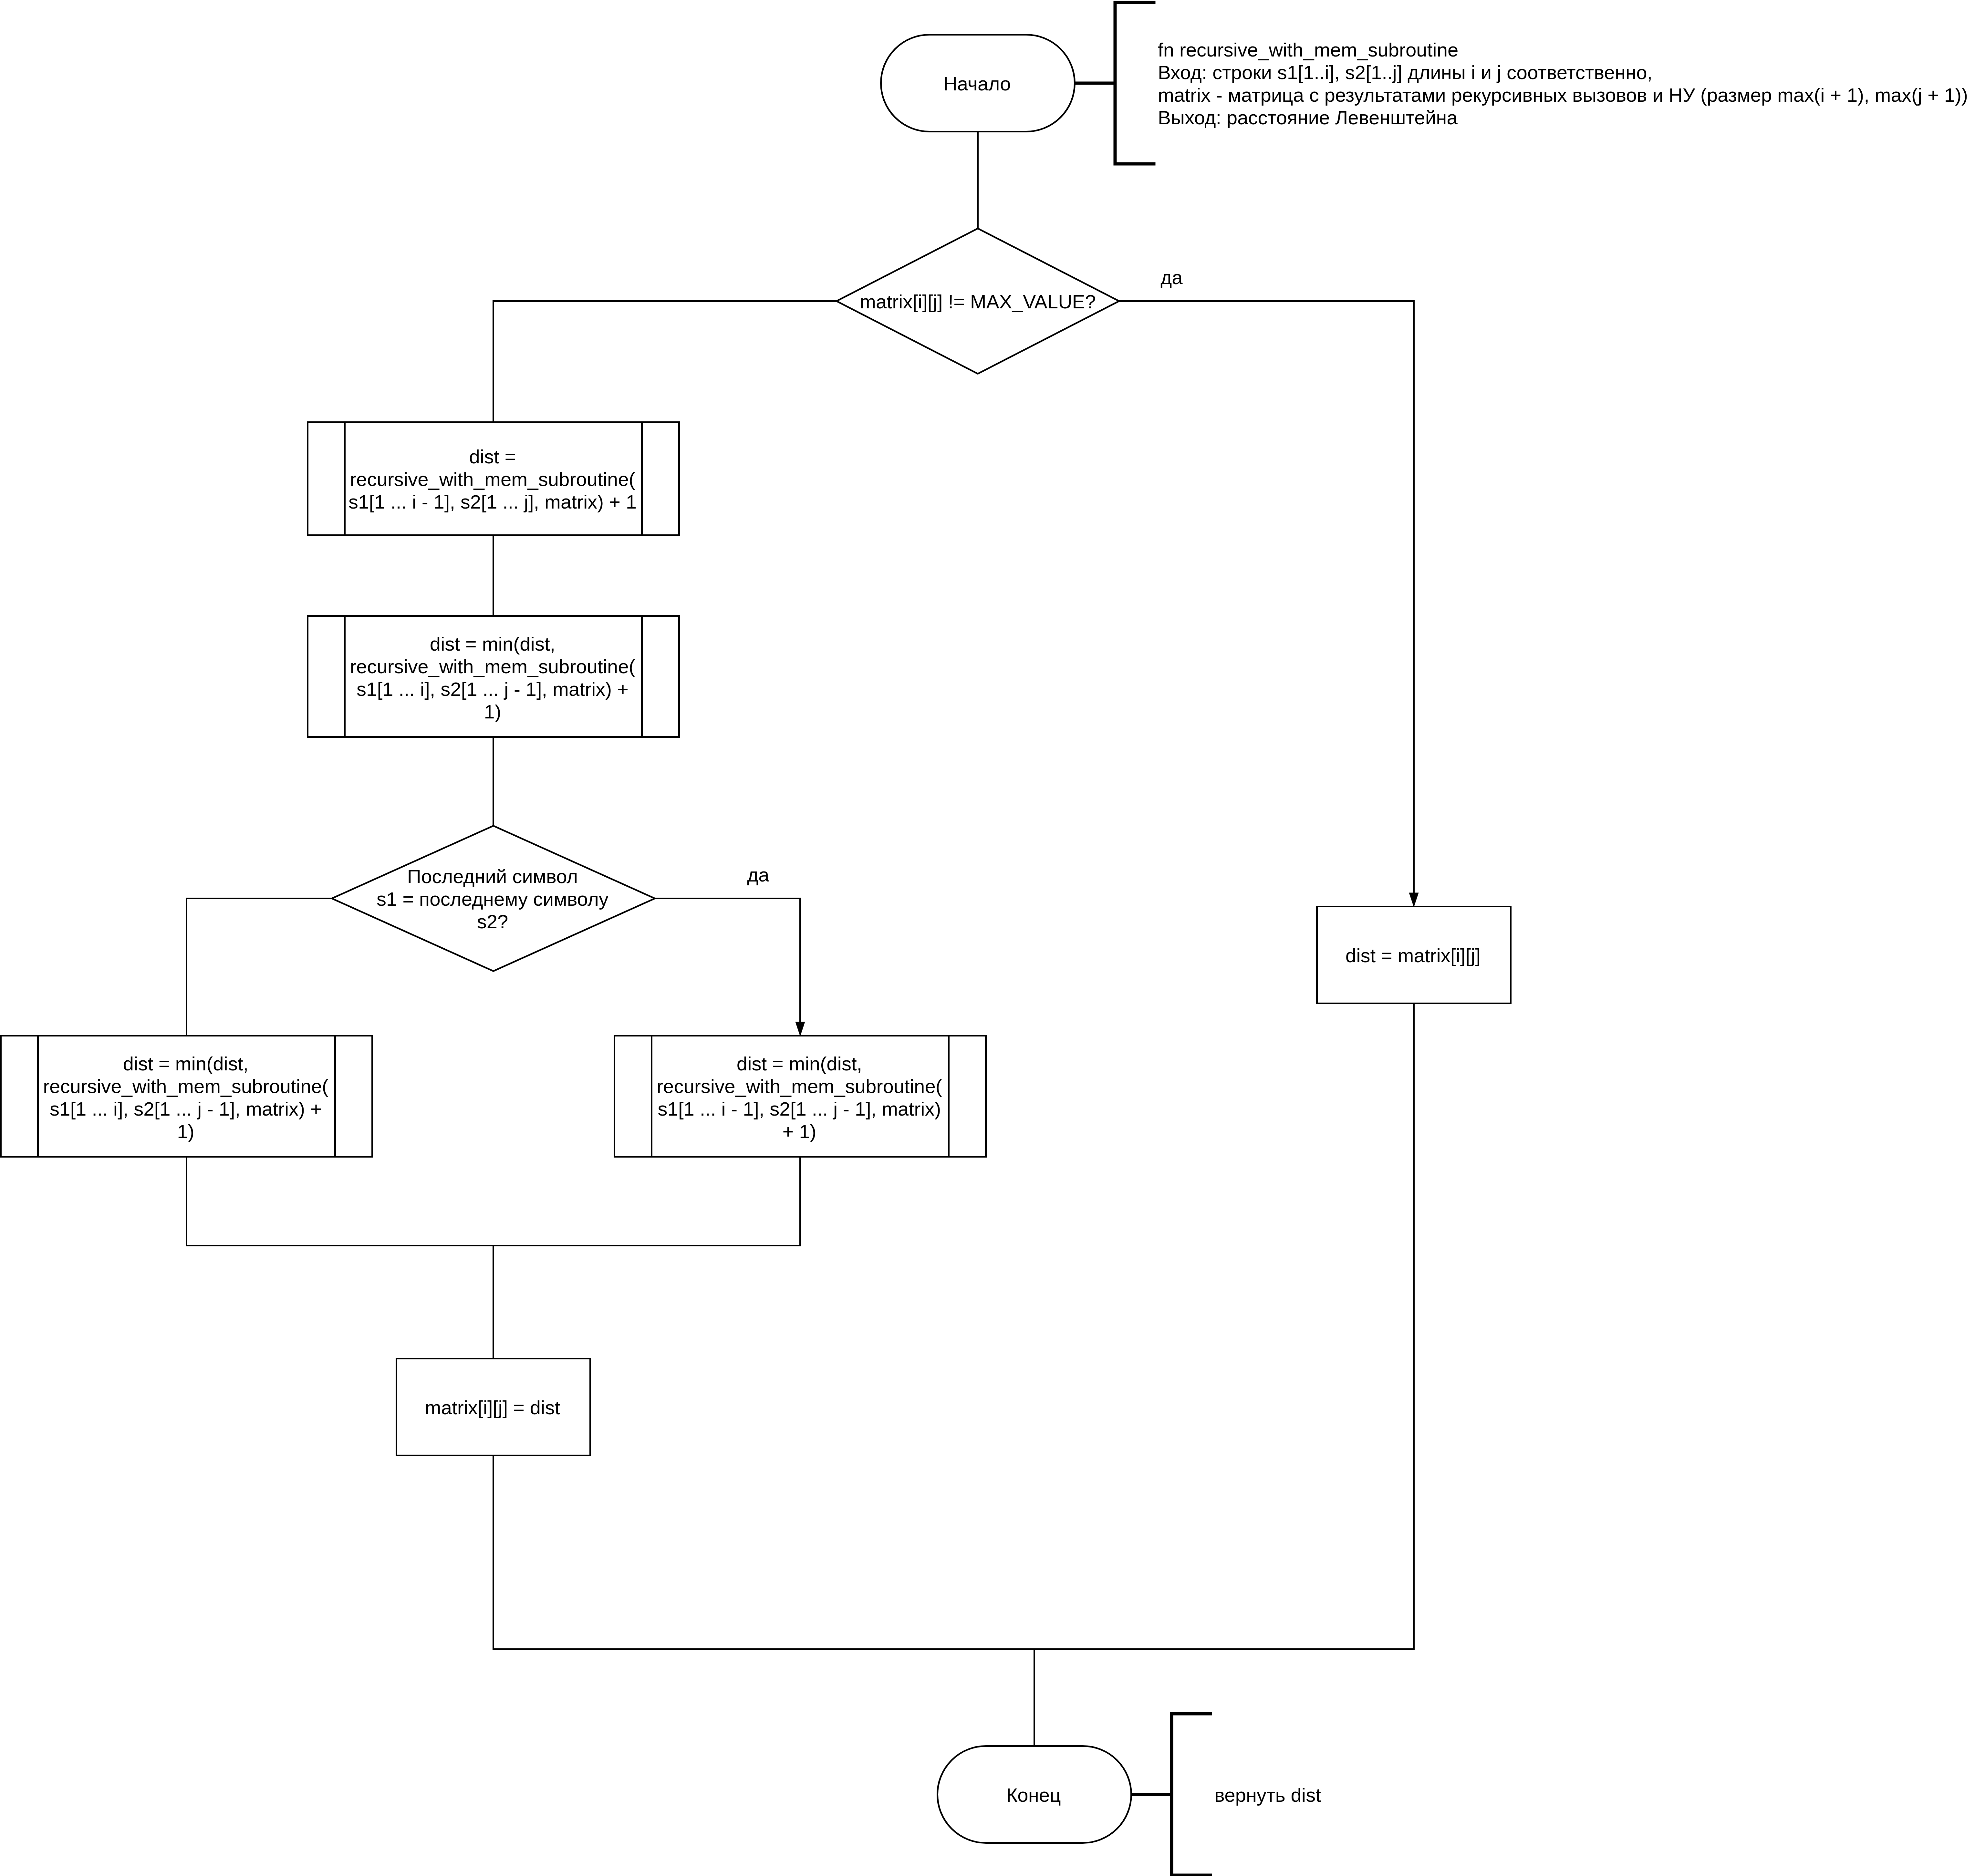
\includegraphics[width=160mm]{images/recursive_with_mem.png}
\caption{Схема матрично-рекурсивного алгоритма нахождения расстояния Дамерау - Левенштейна}
\label{img:recursive_with_mem}
\end{figure}

На рисунке \ref{img:iterative} приведена схема алгоритма нахождения расстояния расстояния Левенштейна с заполнением матрицы.

\begin{figure}
\centering
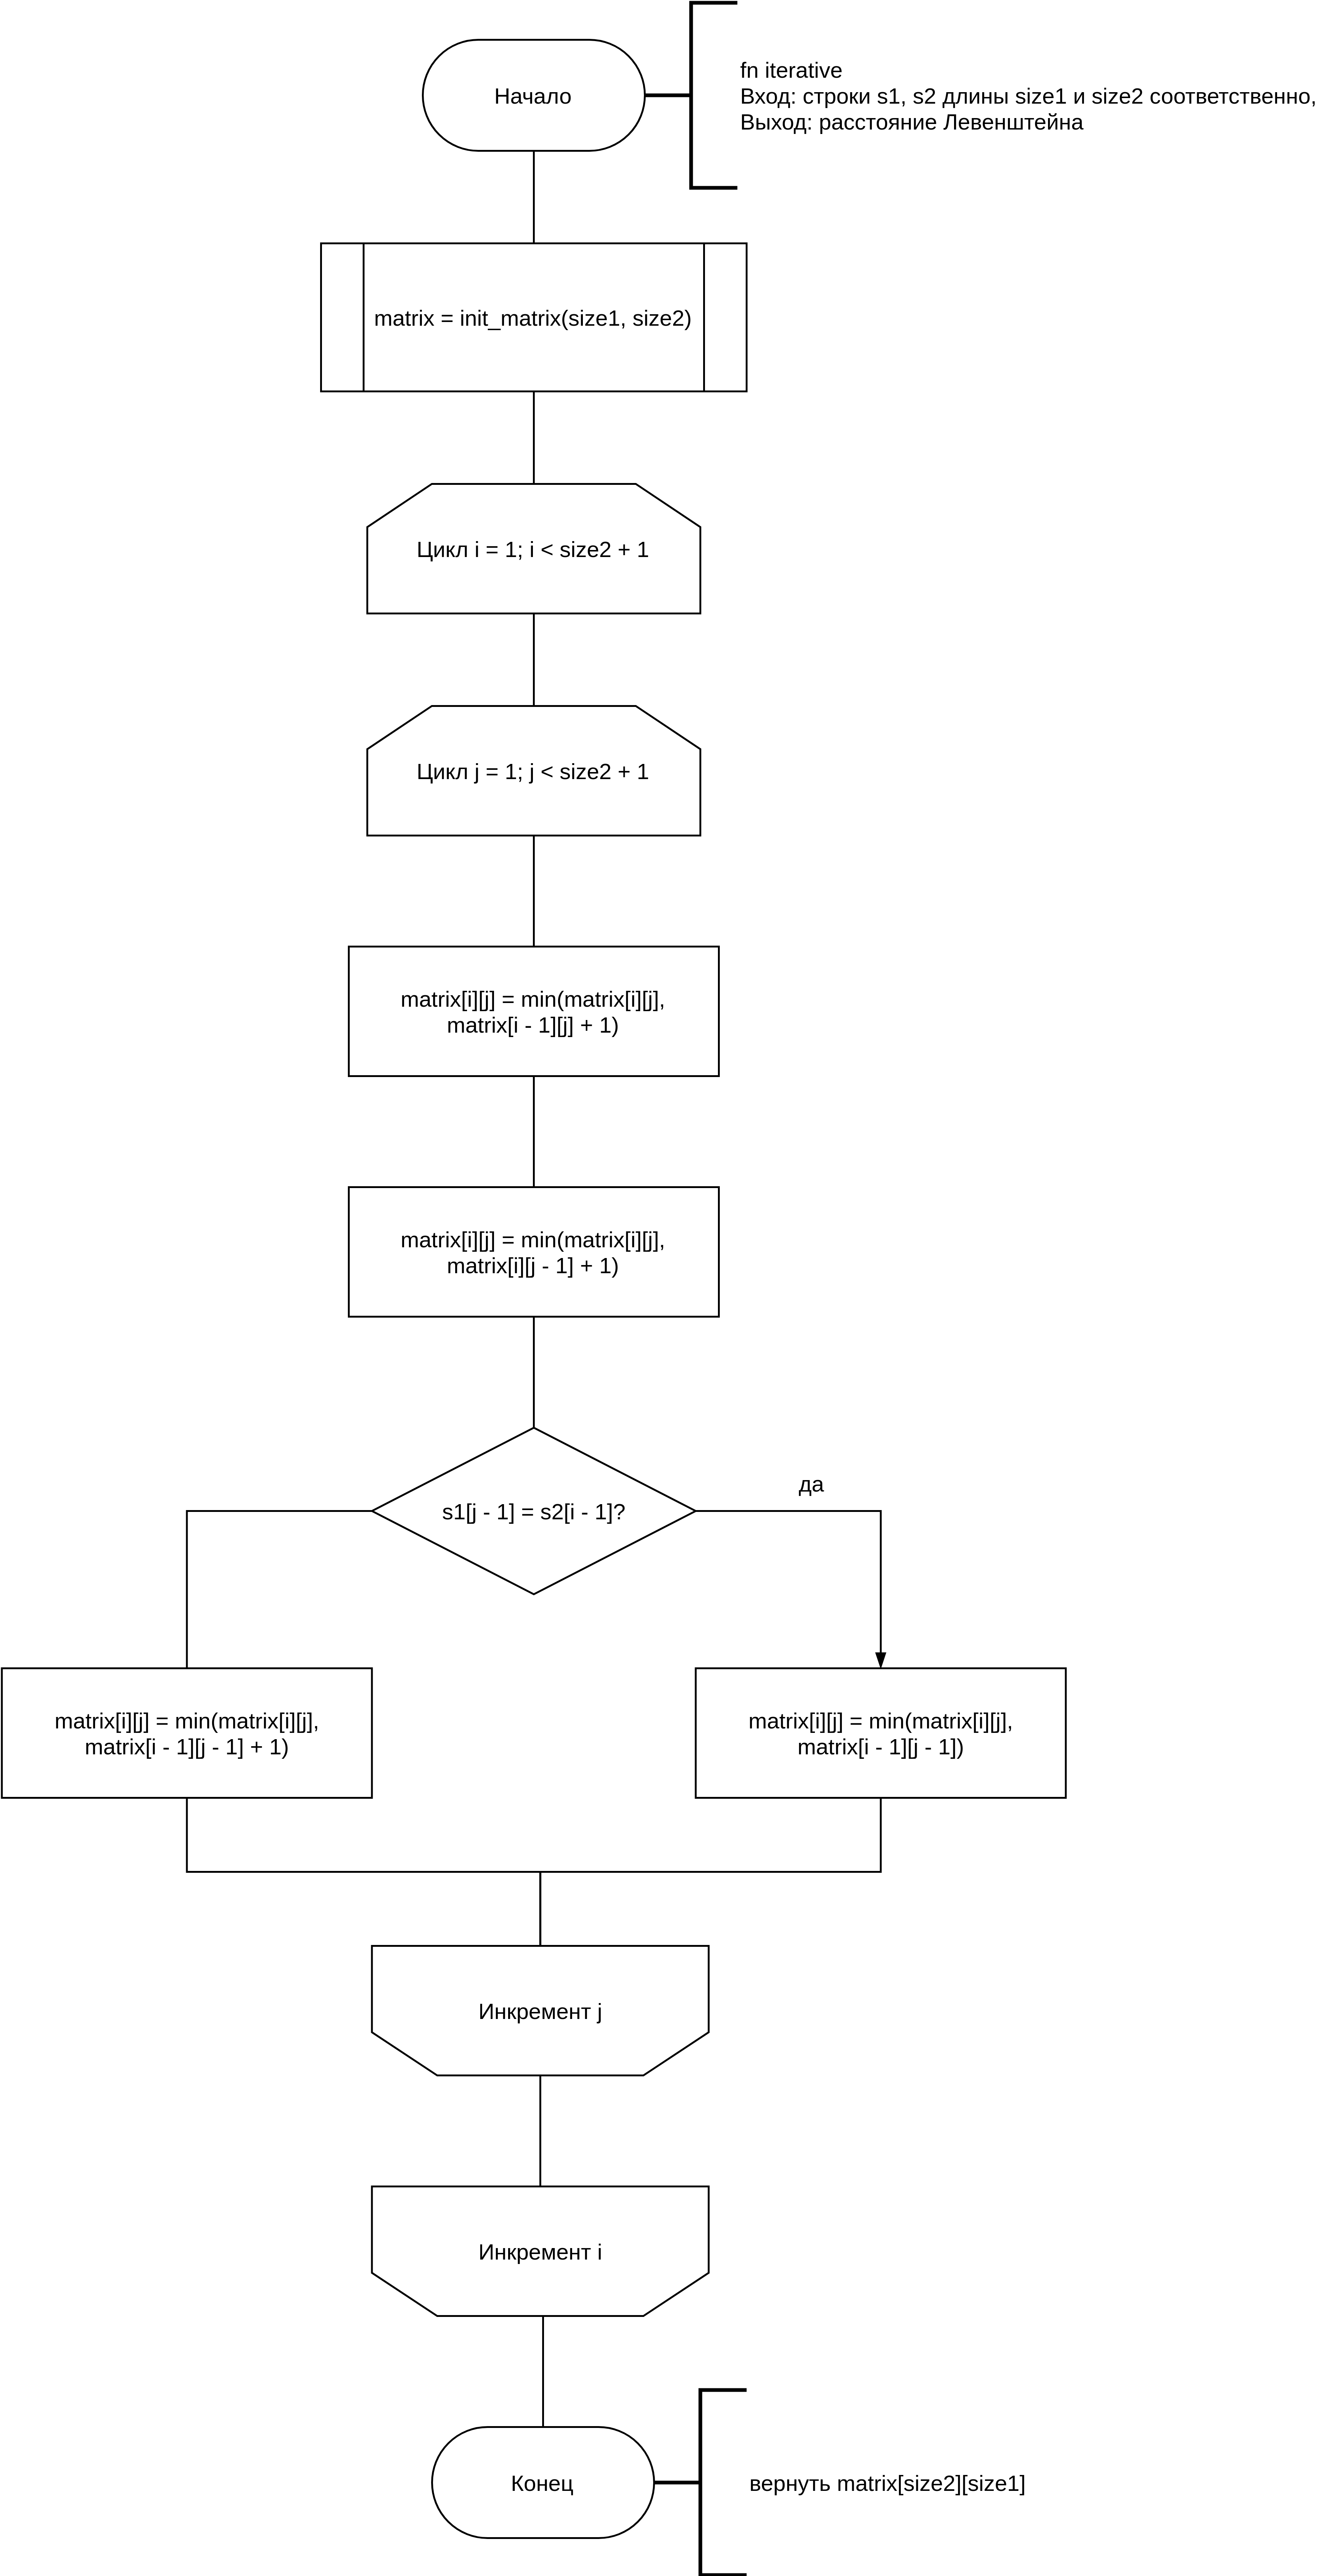
\includegraphics[width=100mm]{images/iterative.png}
\caption{Схема матричного алгоритма нахождения расстояния Левенштейна}
\label{img:iterative}
\end{figure}

\clearpage

\section{Схема алгоритма нахождения расстояния Дамерау — Левенштейна}

На рисунках \ref{img:iterative_dl} и \ref{img:iterative_dl_2} приведена схема матричного алгоритма нахождения расстояния Дамерау - Левенштейна.

\begin{figure}[h]
\centering
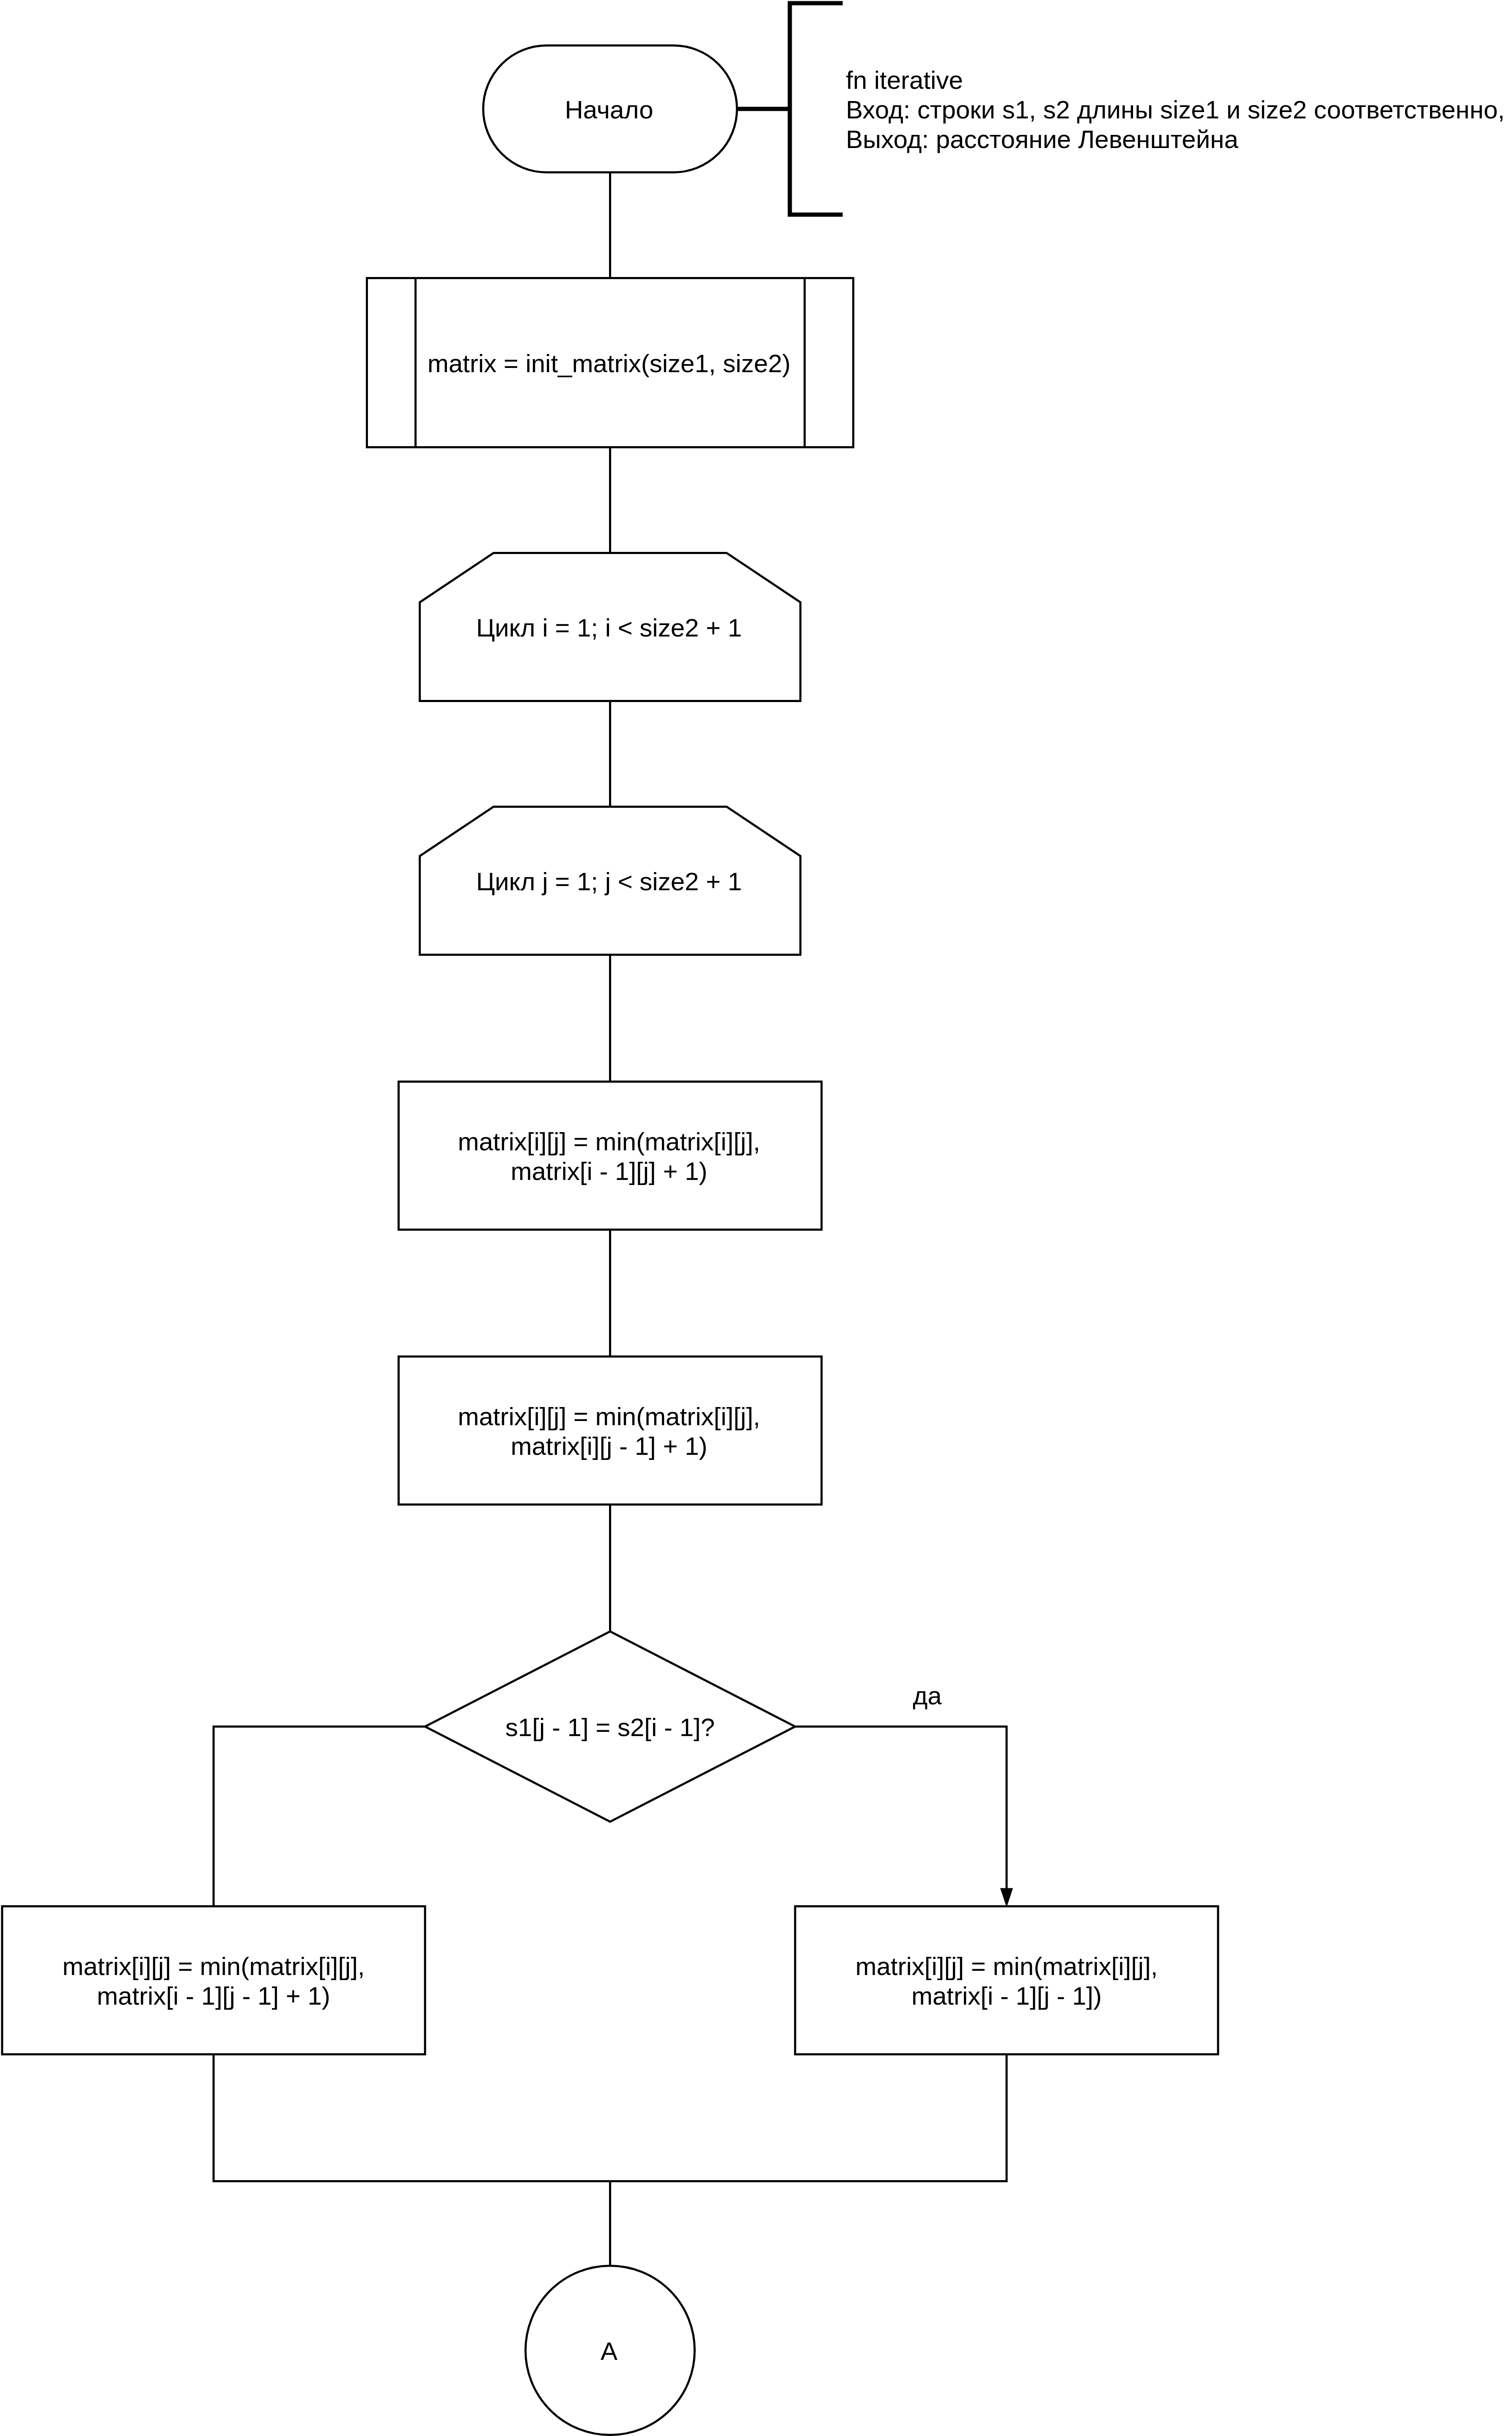
\includegraphics[width=100mm]{images/iterative_dl.png}
\caption{Схема матричного алгоритма нахождения расстояния Дамерау - Левенштейна}
\label{img:iterative_dl}
\end{figure}

\begin{figure}[h]
\centering
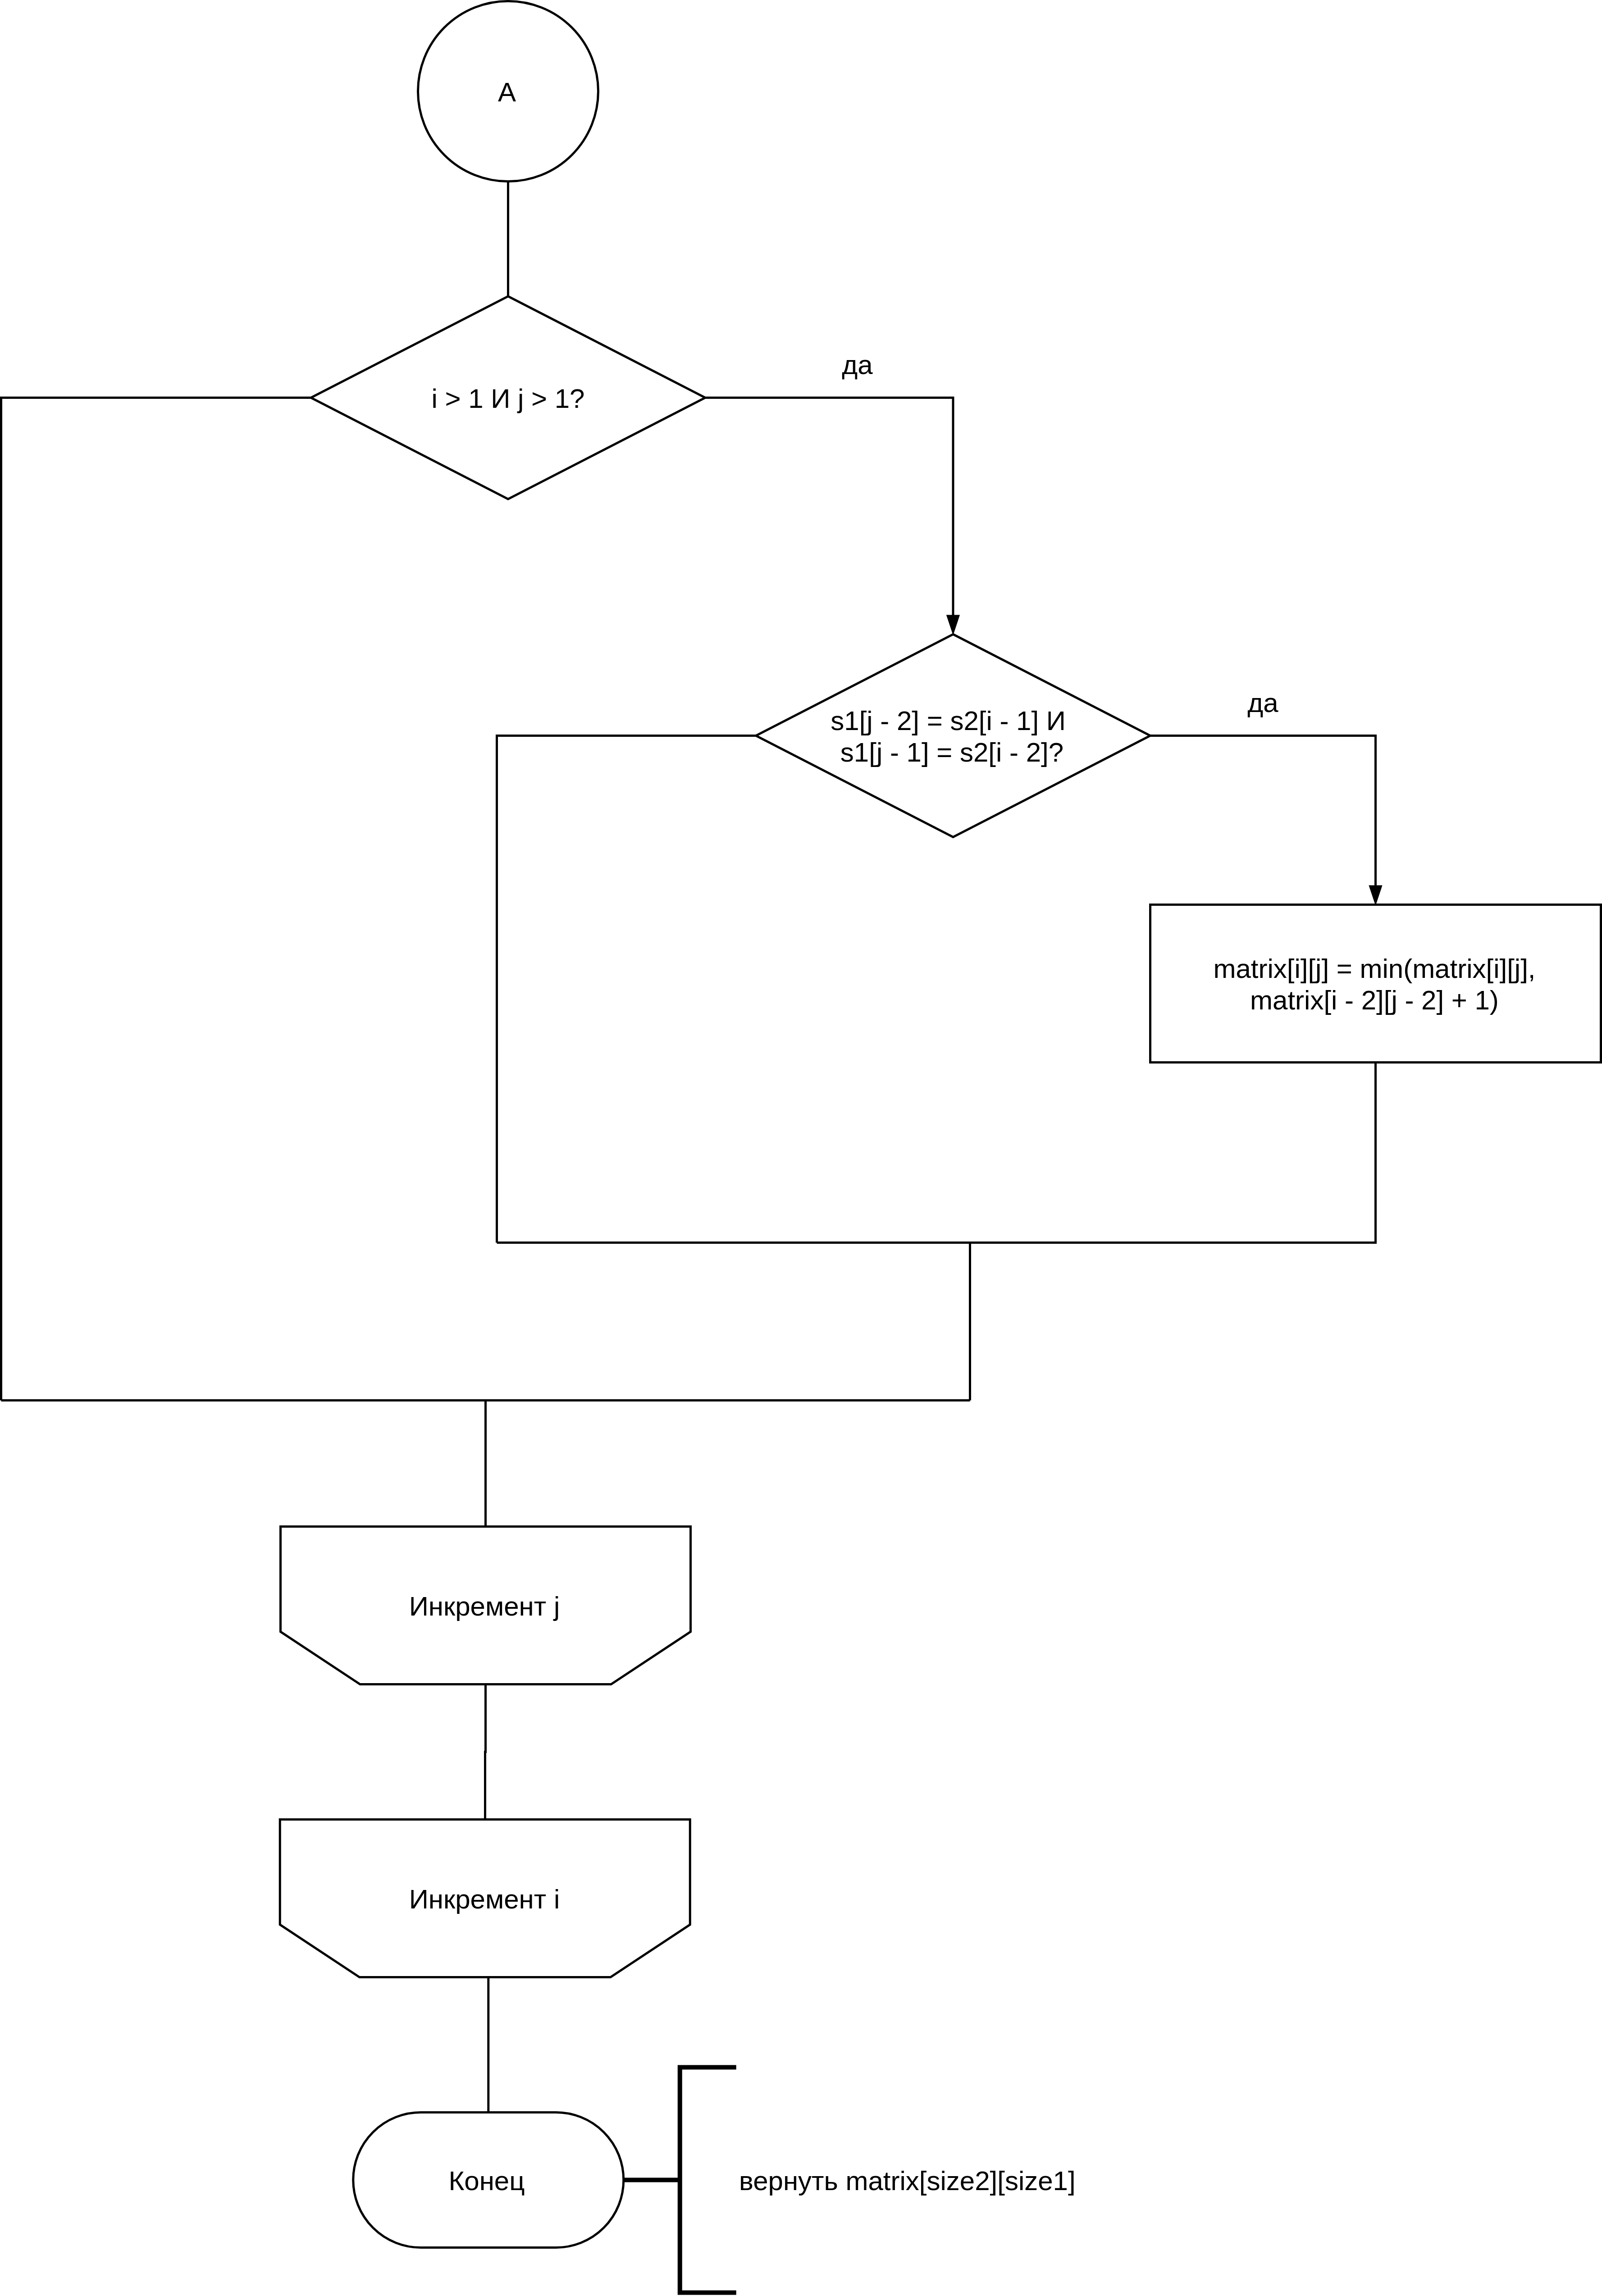
\includegraphics[width=160mm]{images/iterative_dl_2.png}
\caption{Продолжение схемы матричного алгоритма нахождения расстояния Дамерау-Левенштейна}
\label{img:iterative_dl_2}
\end{figure}

\clearpage

\section{Вывод}

На основе теоретических данных, полученных из аналитического раздела были построены схемы требуемых алгоритмов.

\chapter{Технологическая часть}

В данном разделе приведены требования к программному обеспечению, средства реализации и листинги кода.

\section{Требования к ПО}

К программе предъявляется ряд требований:
\begin{itemize}
	\item на вход подаются две строки на английском языке в любом регистре;
	\item на выходе — искомое расстояние для всех четырёх методов и матрицы расстояний для всех методов, за исключением рекурсивного.
\end{itemize}

\section{Средства реализации}

В качестве языка программирования для реализации данной лабораторной работы был выбран ЯП C++. Данный выбор обусловлен наличием большого опыта в написании кода и знанием структуры этого языка программирования.

\section{Демонстрация работы}

\clearpage

\begin{figure}[h]
\centering
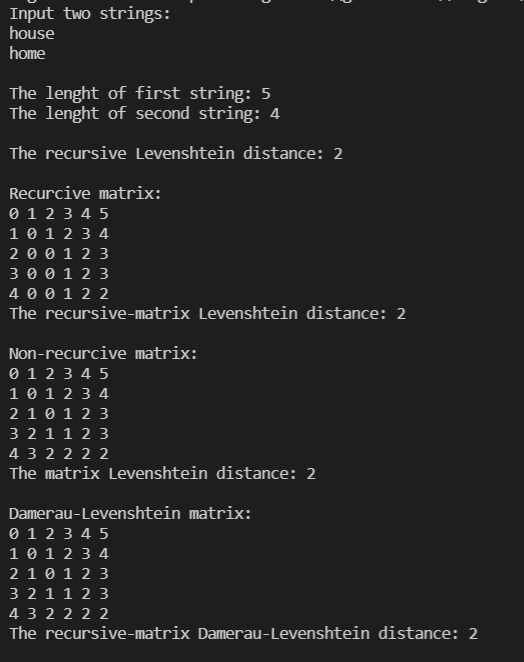
\includegraphics[width=100mm]{images/work.jpg}
\caption{Результат работы программы}
\label{img:iterative_dl}
\end{figure}

\section{Листинг кода}

В листингe \ref{lst:algorithms} приведена реализация алгоритмов нахождения расстояния Левенштейна и Дамерау — Левенштейна, а также вспомогательные функции.

\begin{lstinputlisting}[
	caption={Листинг с алгоритмами},
	label={lst:algorithms},
	style={rust}
]{lab01.cpp}
\end{lstinputlisting}

\clearpage

\section{Вывод}

Были разработаны и протестированы алгоритмы: нахождения расстояния Левенштейна рекурсивно, с заполнением матрицы и матрично-рекурсивно, а также нахождения расстояния Дамерау — Левенштейна с заполнением матрицы.

\chapter{Исследовательская часть}

\section{Технические характеристики}

Технические характеристики устройства, на котором выполнялось тестирование:

\begin{itemize}
	\item Операционная система: Microsoft  Windows 10x86\_64.
	\item Память: 8 ГБ.
	\item Процессор: Intel Core i7-8550U.
\end{itemize}

Тестирование проводилось на ноутбуке, включённом в сеть электропитания. Во время тестирования ноутбук был нагружен только встроенными приложениями окружения, окружением, а также непосредственно системой тестирования.

\section{Время выполнения алгоритмов}

Алгоритмы тестировались при помощи функции \code{GetProccessTime} из \code{Windows.h}.

В листинге \ref{lst:cpu} приведена реализация функции \code{GetProccessTime}.
\begin{lstinputlisting}[
	caption={Листинг с алгоритмами},
	label={lst:cpu},
	style={rust}
]{getCPUTime.c}
\end{lstinputlisting}
\clearpage

% \begin{figure}[h]
% \centering
% \includegraphics[width=160mm]{images/K-tree.png}
% \caption{Скриншот сайта создания строк}
% \label{img:K-tree}
% \end{figure}

В таблице \ref{tabular:functional_test} приведены функциональные тесты для алгоритмов вычисления расстояния Левенштейна и Дамерау — Левенштейна. Все тесты пройдены успешно.

\clearpage

\begin{table}[h]
	\begin{center}
		\caption{\label{tabular:functional_test} Функциональные тесты}
		\begin{tabular}{|c|c|c|c|}
			\hline
			                    &                    & \multicolumn{2}{c|}{\bfseries Ожидаемый результат}    \\ \cline{3-4}
			\bfseries Строка 1  & \bfseries Строка 2 & \bfseries Левенштейн & \bfseries Дамерау — Левенштейн
			\csvreader{images/functional-test.csv}{}
			{\\\hline \csvcoli&\csvcolii&\csvcoliii&\csvcoliv}
			\\\hline
		\end{tabular}
	\end{center}
\end{table}

Результаты замеров приведены в таблице \ref{tbl:time}. В данной таблице для значений, для которых тестирование не выполнялось, в поле результата находится NaN.

\begin{table}[h]
	\begin{center}
		\caption{Замер времени для строк, размером от 10 до 200}
		\label{tbl:time}
		\begin{tabular}{|c|c|c|c|c|}
			\hline
			                      & \multicolumn{4}{c|}{\bfseries Время, нс}                                    \\ \cline{2-5}
			\bfseries Длина строк & \bfseries Recursive & \bfseries RecMem & \bfseries Iterative & \bfseries IterativeDL
			\csvreader{images/time.csv}{}
			{\\\hline \csvcoli&\csvcolii&\csvcoliii&\csvcoliv&\csvcolv}
			\\\hline
		\end{tabular}
	\end{center}
\end{table}

\begin{figure}[h]
	\centering
	\begin{tikzpicture}
		\begin{axis}[
			axis lines=left,
			xlabel=Длина строк,
			ylabel={Время, нс},
			legend pos=north west,
			ymajorgrids=true
		]
			\addplot table[x=len,y=RecursiveMatrix,col sep=comma] {images/time_recmat.csv};
			\addplot table[x=len,y=IterativeMatrix,col sep=comma] {images/time_itmat.csv};
			\legend{Рекурсивный с матрицей, Матричный}
		\end{axis}
	\end{tikzpicture}
	\captionsetup{justification=centering}
	\caption{Зависимость времени работы алгоритма вычисления расстояния Левенштейна от длины строк (рекурсивная с заполнением матрицы и матричная реализации)}
	\label{plt:time_levenshtein}
\end{figure}

\begin{figure}[h]
	\centering
	\begin{tikzpicture}
		\begin{axis}[
			axis lines=left,
			xlabel=Длина строк,
			ylabel={Время, нс},
			legend pos=north west,
			ymajorgrids=true
		]
			\addplot table[x=len,y=IterativeMatrix,col sep=comma] {images/time_itmat.csv};
			\addplot table[x=len,y=DamerauLevenshtein,col sep=comma] {images/time_dl.csv};
			\legend{Левенштейн, Д. — Левенштейн}
		\end{axis}
	\end{tikzpicture}
	\captionsetup{justification=centering}
	\caption{Зависимость времени работы матричных реализаций алгоритмов нахождения расстояний Левенштейна и Дамерау — Левенштейна}
	\label{plt:time_dl}
\end{figure}


\section{Использование памяти}

Алгоритмы нахождения расстояний Левенштейна и Дамерау — Левенштейна не отличаются друг от друга с точки зрения использования памяти, следовательно, достаточно рассмотреть лишь разницу рекурсивной и матричной реализаций этих алгоритмов.

Максимальная глубина стека вызовов при рекурсивной реализации равна сумме длин входящих строк, при этом для каждого вызова рекурсии в моей реализации требуется:
\begin{itemize}
    \item 4 локальные перeменные беззнакового типа, в моем случае: $4 \cdot 8 = 32$ байта;
    \item 2 аргумента типа строка: $2 \cdot 16 = 32$ байта;
    \item адрес возврата: 8 байт;
    \item место для записи возвращаемого функцией значения: 8 байт.
\end{itemize}
Таким образом получается, что при обычной рекурсии на один вызов требуется (\ref{for:onecall}): 

\begin{equation}
M_{per call} = 32 + 32 + 8 + 8 = 80 байт
\label{for:onecall}
\end{equation}

Следовательно память, расходуемая в момент, когда стек вызовов максимален, равна (\ref{for:rec}): 

\begin{equation}
    M_{recursive} = 80 \cdot depth
\label{for:rec}
\end{equation}

где \textit{depth} - максимальная глубина стека вызовов, которая равна (\ref{for:depth}):

\begin{equation}
depth = |S_1| + |S_2|
\label{for:depth}
\end{equation}

где $S_1, S_2$ - строки.

Если мы используем рекурсивный алгоритм с заполнением матрицы матрицы, то для каждого вызова рекурсии добавляется новый аргумент - ссылка на матрицу - размером $8$ байт. Также в данном алгоритме требуется память на саму матрицу, размеры которой: $m = |S_1| + 1, n = |S_2| + 1$. Размер элемента матрицы равен размеру беззнакового целого числа, используемого в моей реализации, то есть $8$ байт. Отсюда выходит, что память, которая тратится на хранение матрицы (\ref{for:matrix}):
\begin{equation}
M_{Matrix} = (|S_1| + 1) \cdot (|S_2| + 1) \cdot 8
\label{for:matrix}
\end{equation}

Таким образом, при рекурсивной реализации требуемая память равна (\ref{for:rec_mem}):
\begin{equation}
M_{recursive} = 88 \cdot depth + M_{Matrix}
\label{for:rec_mem}
\end{equation}
где $M_{Matrix}$ взято из соотношения \ref{for:matrix}.

Память, требуемая для при итеративной реализации, состоит из следующего:
\begin{itemize}
    \item 4 локальные перeменные беззнакового типа, в моем случае: $4 \cdot 8 = 32$ байта;
    \item 2 аргумента типа строка: $2 \cdot 16 = 32$ байта;
    \item адрес возврата: 8 байт;
    \item место для записи возвращаемого функцией значения: 8 байт;
    \item матрица: $M_{Matrix}$ из соотношения \ref{for:matrix}.
\end{itemize}

Таким образом общая расходуемая память итеративных алгоритмов (\ref{for:iter}):

\begin{equation}
M_{iter} = M_{Matrix} + 80
\label{for:iter}
\end{equation}

где $M_{Matrix}$ определяется из соотношения \ref{for:matrix}.

\section{Вывод}

Рекурсивный алгоритм нахождения расстояния Левенштейна работает на порядок дольше итеративных реализаций, время его работы увеличивается в геометрической прогрессии. На словах длиной 10 символов, матричная реализация алгоритма нахождения расстояния Левенштейна превосходит по времени работы рекурсивную на несколько порядков. Рекурсивный алгоритм с заполнением матрицы превосходит простой рекурсивный и сравним по времени работы с матричными алгоритмами. Алгоритм нахождения расстояния Дамерау — Левенштейна по времени выполнения сопоставим с алгоритмом нахождения расстояния Левенштейна. В нём добавлена дополнительная проверка, позволяющая находить ошибки пользователя, связанные с неверным порядком букв, в связи с чем он работает незначительно дольше, чем алгоритм нахождения расстояния Левенштейна.

\chapter*{Заключение}
\addcontentsline{toc}{chapter}{Заключение}

В ходе выполнения лабораторной работы была проделана следующая работа:

\begin{itemize}
    \item были теоретически изучены алгоритмы нахождения расстояний Левенштейна и Дамерау--Левенштейна;
	\item для некоторых реализаций были применены методы динамического программирования, что позволило сделать алгоритмы быстрее;
	\item были практически реализованы алгоритмы в 2 вариантах: рекурсивном и итеративном;
	\item на основе полученных в ходе экспериментов данных были сделаны выводы по поводу эффективности всех реализованных алгоритмов;
	\item был подготовлен отчёт по ЛР.
\end{itemize}

\chapter*{Список литературы}

[1] Левенштейн В. И. Двоичные коды с исправлением выпадений, вставок
и замещений символов. — М.: Доклады АН СССР, 1965. Т. 163. С. 845-
848.

[2] Процессор Intel Соrе"" 17-85500 [Электронный ресурc] Режим доступа: https://ark.intel.com/content/www/ru/ru/ark/products/122589/intel-core-i7-8550u-processor-8m-cache-up-to-4-00-ghz.html
(дата обращения: 14.09.2021)

[3] ЛаТеХ для продвинутых: Как контролировать положение плавающих объектов "floats"? [Электронный ресурc] Режим доступа: http://mydebianblog.blogspot.com/2013/03/amorua-advanced-floats.html (дата обращения: 01.10.2021)

[4] GetProcessTimes function (processthreadsapi.h) [Электронный ресурc] Режим доступа: https://docs.microsoft.com/en-us/windows/win32/api/processthreadsapi/nf-processthreadsapi-getprocesstimes#syntax (дата обращения: 27.09.2021)

[5] WIndows 10 [Электронный ресурc] Режим доступа: https://www.microsoft.com/ru-ru/windows/get-windows-10 (дата обращения: 14.09.2021)

\end{document}